\documentclass[]{standalone}
\usepackage{tikz}
\usepackage{palatino}
\usetikzlibrary{shapes,arrows,trees,calc}
\usepackage{tikz}
\usetikzlibrary{trees,shapes}
\begin{document}
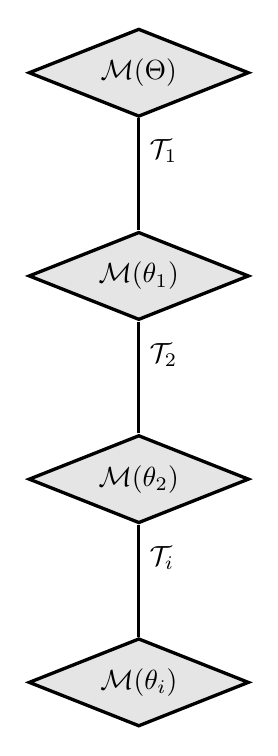
\begin{tikzpicture}[
    test/.style={
        % Node style
        diamond, 
        aspect=2.5,
        very thick,
        draw=black,
        fill=gray!20,
        text width=1.1cm,
        align=center, 
        anchor=north},
    dec/.style={
        rectangle,
        very thick,
        draw=black,
        fill=gray!50,
        text width=2cm,
        text centered, 
        anchor=north
    },
    % Children and edges style
    edge from parent/.style={
        very thick,
    draw=black},
    edge from parent fork down,
    level 1/.style={
        sibling distance=4cm,
        level distance=2cm}
    ]

\node (t1) [test] {$\mathcal{M}(\Theta)$} 
    child { node (t2) [test] {$\mathcal{M}(\theta_1)$}  
        child { node (t3) [test] {$\mathcal{M}(\theta_2)$} 
            child { node (t4) [test] {$\mathcal{M}(\theta_i)$}
             edge from parent node [right] {$\mathcal{T}_i$} }edge from parent node [right] {$\mathcal{T}_2$}}edge from parent node [right] {$\mathcal{T}_1$}} %
;
\end{tikzpicture}
\end{document}
